\documentclass[%
%letter,
reprint,
%preprint,
%superscriptaddress,
%groupedaddress,
%unsortedaddress,
%runinaddress,
%frontmatterverbose,
%preprintnumbers,
%nofootinbib,
%nobibnotes,
%bibnotes,
amsmath,amssymb,
aps,
%pra,
%prb,
%longbibliography,
%rmp,
%prstab,
%prstper,
%floatfix,
]{revtex4-2}
%========================package=====================

\usepackage{graphicx}% Include figure files
\usepackage{dcolumn}% Align table columns on decimal point
\usepackage{bm}% bold math
\usepackage[colorlinks=true,linkcolor=blue,anchorcolor=blue, citecolor=blue,urlcolor=blue]{hyperref}% add hypertext capabilities
\usepackage[mathlines]{lineno}% Enable numbering of text and display math

\begin{document}
%======================== head
\title{Pressure-enhanced robustness of helical edge state in ABA Tri-layer Graphene}% Force line breaks with \\
\author{Shijie Fang$^1$}
\author{Hua Fan$^2$}
\author{Jifeng Shao$^1$}
\author{Yue Zhao$^{1,2,3}$}
\email{Author1 e-mail}
\affiliation{
1 Shenzhen Institute for Quantum Science and Engineering (SIQSE), Southern University of Science and Technology (SUSTech), China
}
\affiliation{2 Department of Physics, SUSTech, China}
\affiliation{3 International Quantum Academy, Shenzhen, Guangdong 518048, China}
%\date{\today}
%=======================Abstract=====================
\begin{abstract}

    Multi-layer graphene systems are promising platforms to study interesting physical phenomena, 
    including unique quantum hall physics, spontaneous symmetry breaking, and topological properties. 
    Here, by applying hydrostatic pressure on the tri-layer ABA graphene, 
    the phase diagram at the charge neutrality point undergoes a significant change, 
    indicating a complicated interplay among different energy scales. 
    Also, quantum parity hall state, a kind of helical edge state protected by mirror symmetry, emerges after pressure.
    The measured Landau Fan diagram illustrates the modification of the band structure by pressure, 
    which can be used to explain the observed phenomenon.
        
\end{abstract}

\maketitle
%\tableofcontents
%========================Introduction==================== 
\section*{Introduction}
%\tableofcontents
%========================Introduction====================
Regarding multilayer graphene systems, their rich physical properties make them widely regarded as a platform 
for studying unconventional properties of two-dimensional electron systems. 
Up to now, many intriguing physical phenomena has been found in multilayer graphene systems, ranging from single-particle to many-body physics, 
such as the Lifshitz transition of Fermi surface topology \cite{shi2018tunable, bao2011stacking}, 
Landau level physics in the single-particle picture \cite{taychatanapat2011quantum, campos2016landau, che2020substrate, shimazaki2016landau},
quantum hall ferromagnetism even fractionalization under a high perpendicular magnetic field 
\cite{zhang2012hund, young2012spin, liu2022visualizing, coissard2022imaging, hunt2013massive, yu2014hierarchy, hunt2017direct, lee2014chemical, lee2013broken, stepanov2016tunable, datta2017strong}, 
and various symmetry broken states near charge neutrality and under a relatively small magnetic field \cite{weitz2010broken, stepanov2019quantum, zibrov2018emergent, winterer2022spontaneous}. 
Besides these phenomena, insulating bulk states with non-trivial edge channels can emerge in various graphene systems under different conditions, including chiral and helical edge states 
\cite{zhang2011spontaneous, young2014tunable, veyrat2020helical, geisenhof2021quantum, maher2013evidence, spanton2018observation, stepanov2019quantum, winterer2023ferroelectric, han2023correlated}.

Among them, tri-layer ABA graphene has attracted widespread attention due to its unique band structure at low energy regime. 
As a highly tunable platform, it provides an excellent opportunity to study its single-particle band structure and many-body phenomenon. 
In previous studies, its electronic properties have been studied by tuning multiple control knobs like carrier density, displacement field, and magnetic field, 
which lead to many interesting discoveries in this system \cite{taychatanapat2011quantum, campos2016landau, shimazaki2016landau, che2020substrate, bao2011stacking, stepanov2016tunable, lee2013broken, stepanov2019quantum, zibrov2018emergent, datta2017strong}.
Notably, because the low-energy band structure of multilayer graphene is highly sensitive to the interlayer hopping strength, 
applying hydrostatic pressure to reduce the interlayer distance and further study its properties has become a highly promising research approach. 

In recent years, condensed matter physics has witnessed a growing interest in exploring the topologically non-trivial edge states in materials. 
As an extension of the chiral edge state, the helical edge state is a special boundary state featured by the non-dissipative channels with opposite motion directions. 
Helical conductors have been proposed to realize Majorana statistics for quantum computation \cite{qi2011topological, hasan2010colloquium, oreg2010helical, lutchyn2010majorana}.
Since its first theoretical proposed \cite{kane2005quantum, kane2005z}, multiple ways are developed to achieve helical edge states, 
including topologically non-trivial band structures protected by time-reversal symmetry, such as those found in QSHE systems \cite{bernevig2006quantum, roth2009nonlocal}. 
In addition, in those systems where the conduction band is energetically below the valence band, the introduction of a magnetic field can cause the crossing of “hole-like” Landau levels with “electron-like” Landau levels at the system's boundary, 
leading to the emergence of spin-degenerate helical edge states which are composed of opposite-propagating chiral edge states.
The advent of multilayer graphenes has provided a fertile platform for exploring different types of helical edge states 
because of the unique band structure near the charge neutrality point (CNP). 
Many experimental evidence has confirmed the existence of helical edge states in multilayer graphene systems, ranging from monolayer to tetralayer graphene
\cite{veyrat2020helical, young2014tunable, maher2013evidence, stepanov2019quantum, che2020helical}.
% \cite{veyrat2020helical, young2014tunable, maher2013evidence, li2019metallic, stepanov2019quantum, che2020helical}.

Here we report the dramatic change of phase diagram at the charge neutrality point and the emergence of a kind of helical edge state, named quantum parity hall effect, after applying 1.0 GPa hydrostatic pressure.
Tri-layer ABA graphene is one of the material platforms which can hold helical edge states owing to its unique band structure.
The low-energy band structure of tri-layer ABA graphene consists of a monolayer-like valence band and a bilayer-like conduction band in the absence of displacement field, which have an energy overlap, as shown in Figure~\ref{fig:1}(b). 
Both branches are protected by mirror symmetry and have odd(monolayer) or even(bilayer) parity. However, when a displacement field is applied, they mix due to the breaking of mirror symmetry.
~\\

\section*{Method and Characterization}
%\tableofcontents
%========================Method====================

Here, we fabricate the tri-layer ABA device that has high mobility for observing its quantum hall effect, and we changed its band structure and phase diagram by exerting hydrostatic pressure out of the plane.
Our device is a high-quality dual-gate device with a Hall-bar geometry, with hexagonal boron nitride(h-BN) as the dielectric spacer and few-layer graphite as the top and bottom gates, 
which is stacked together using a dry-transfer method \cite{wang2013one}. 
In detail, the tri-layer ABA graphene is encapsulated by two hBN sheets whose geometric capacitances are $C_t, C_b$, respectively, in the unit of $V^{-1}·cm^{-2}$. 
Moreover, outside of hBN sheets, two graphite stacks act as top and bottom gates. 
By modulating the top gate voltage $V_t$ and bottom-gate voltage $V_b$, the carrier density $n(10^{12}cm^{-2})$ and out-of-plane displacement field $D(V/nm)$ can be tuned continuously, 
according to the relation:
\begin{equation}
    \begin{split}
        n &= C_t V_t + C_b V_b \\
        D &= \frac{1}{2\epsilon_0}(C_t V_t - C_b V_b)
    \end{split}
    \label{eq:nD_formula}
\end{equation}
with $\epsilon_0$ the vacuum permittivity. 
So, this configuration enables us to measure its transport properties with multiple in-situ tunable external parameters.

We also utilized hydrostatic pressure to reduce the interlayer distance and strengthen the interlayer coupling.
It can change the material structure of Van der Waals(VdW) material systems without enhanced disorder effect, thanks to their weak out-of-plane VdW bonding.
Previous work shows that hydrostatic pressure can compress the interlayer distance of graphene superlattice by $5\%$ with less than 2.5 GPa\cite{yankowitz2018dynamic} and can induce superconductivity in twisted bilayer graphene away from magic angle\cite{yankowitz2019tuning}. Therefore, hydrostatic pressure is a powerful tool for tuning the electronic structure effectively.
Here, we mainly investigate the change of the device under a 1.0 GPa hydrostatic pressure by comparing it to that in ambient pressure.

The high quality of this device can be verified by the dependence of longitudinal resistance as a function of n and D. 
An external out-of-plane displacement field opens a gap at the charge neutrality point, schematically shown in Fig.~\ref{fig:1}(b). 
Fig.~\ref{fig:1}(c) and (d) show the resistance of the device at zero magnetic fields before and after pressurization. 
It is found that, along the charge neutrality point, the resistance of both increases dramatically, which indicates the appearance of an electric-field-induced band gap. 
This signature reflects a good quality and low disorder of our device before and after pressurization, which enables us to study the sample's band structure using the Landau fan diagram 
under an out-of-plane magnetic field.

In this work, transport measurements were conducted on this tri-layer ABA graphene device before and after 1.0 GPa pressure at a temperature T = 1.6K, and our findings are three-fold. 
Firstly, we explore the phase diagram of the tri-layer ABA graphene at the charge neutrality point as a function of the magnetic field and displacement field, 
by making a slow scan of the displacement field around and magnetic field around. 
The one after pressure reveals a complex competition between different energy scales. 
Interestingly, we observe the signatures of some helical edge state after pressure, indicated by its nearly quantized four-terminal longitudinal conductance and near-zero transverse resistance. 
This state fades away when D is large enough, demonstrating that it is protected by mirror symmetry, which is broken under a finite D field. 
Secondly, in order to partially explain the observed phenomenon above, we perform the magneto-transport measurement to investigate how the pressure modifies the hopping parameters. 
Specifically, the Landau fan diagram shows that the crossing points among Landau levels undergo a significant shift, appearing at a larger magnetic field at 1.0 GPa pressure. 
This phenomenon indicates that the strength of interlayer hopping, alternatively, the low energy band structure, can be modified by pressure. 
Finally, our magneto-transport measurement finds some signatures of the four-fold quasi-degenerate zeroth monolayer-like Landau levels, which cannot be explained under the single-particle picture. 
These signatures include the complete splitting of these degenerate Landau levels at a relatively high magnetic field (about 10 T) before and after pressure. 
Besides, we found the Landau level splitting at the intermediate magnetic field only after pressurization. 
These two signatures indicate that the enlarged Landau level gaps, which are inconsistent with the single particle picture, should be associated with enhancing interlayer exchange interaction.

~\\
% ~\\
\section*{Results}
\subsection*{{\color{red} Phase diagram of $\nu=0$ at small B}}
% Phase diagram of $\nu=0$ at small B
We first investigate the phase diagram of tri-layer ABA graphene around the charge neutrality point by measuring the four-terminal longitudinal conductance $G_{xx}(\frac{e^2}{h})$ 
under a small magnetic field and displacement field. Figure~\ref{fig:2}(a) and ~\ref{fig:2}(b) show this before and after pressure. 
As can be seen, the phase diagram at 1 GPa reveals a very different phase diagram than that at 0 GPa.

Firstly, the phase diagram at 0 GPa is similar to that observed in \cite{stepanov2019quantum}. 
The conductance around B = 0T and D = 0 V/nm is the highest because of the metallic property caused by the overlap between the valence and conduction bands. 
As |D| increases, opening a band gap at the charge neutrality point leads to a quick decrease of $G_{xx}$, indicating the high quality of our sample. 
In addition, along the D = 0 V/nm line profile, a local minimum of $G_{xx}$ emerges around B = 0.25T, indicated by the green arrows, surrounded by a high-conductance ring. 
This signature demonstrates that the nature of this state is different from that at higher B or zero B.
This phase diagram is similar to that of \cite{stepanov2019quantum}.
In the latter, this behaviour is interpreted as the emergence of “Quantum Parity Hall State” (QPH), which has nearly quantized four-terminal longitudinal conductance. 
However, here, we do not observe these well-defined features to claim its edge state configuration, so it should be regarded as an incipient of QPH, 
demonstrating it is not very stable at a temperature as high as T = 1.6K. In contrast, the temperature in \cite{stepanov2019quantum} is 0.4K.

However, at 1 GPa, the phase diagram becomes very different: the high-conductance state near B = 0T and D = 0V/nm has shrunk into a much smaller region, and more features appear as B and D changes. 
The first interesting feature is the appearance of spikes of longitudinal conductance $G_{xx}(B, D)$ within a small range of B $\in$ [0.3T, 0.8T], 
marked by the dashed-line trajectories of different colours in Figure~\ref{fig:2}(b). 
These features refer to the phase boundaries of first-order phase transitions, which are accompanied by a sudden change of charge distribution among several flavours \cite{zondiner2020cascade}, 
driven by the competition between displacement field and magnetic field. 
Similar transport signatures have been found in bilayer graphene and rhombohedral tri-layer graphene, 
but requires larger magnetic field \cite{geisenhof2021quantum, weitz2010broken, maher2013evidence, winterer2023ferroelectric}. 
We find that one of the phase boundaries displays a parabolic-like trajectory at low B (marked by a purple dashed line) and a linear trajectory at high B (marked by a green dashed line), 
another one also displays a linear behaviour (marked by an orange dashed line). 
These boundaries demonstrate the competition between different energy scales. 
Based on these phase boundaries and other features, we can divide the phase diagram at the charge neutrality point into several regions, 
and four of them are labelled as A, B, C and D, as shown in Figure~\ref{fig:2}(c).

The phase boundary between phase A and phase B can be explained by the competition between exchange interaction caused by B and layer polarization driven by D, 
since the exchange interaction proportional to $\frac{e^2}{l_B}\sim \sqrt{B}$ whereas the layer polarization characterized by $\Delta_1=\alpha dD$, 
with $\alpha\approx 0.3$ the empirical parameters describing the screening effect 
and $d\approx 0.3nm$ the nearest interlayer distance. Following the analysis of \cite{zhang2012hund, stepanov2019quantum}, 
one role of the magnetic field is to tune the exchange interaction strength, whereas the displacement field favours a layer polarization. 
It is reasonable that these energy scales drive the competition between phase A and phase B. 
In contrast, the phase boundary between phase C and phase B or phase D and phase B, displays a linear-shape trajectory, indicating a different mechanism from that between phase A and phase B. 
This linear dependence indicates that the energy scale associated with B should also be linear with B. 
From some theoretical work \cite{zhang2012hund}, the Zeeman energy $E_{ZM}$, the difference between intralayer and interlayer exchange interaction $\delta E_{ex}$ and electrostatic energy $E_H$ are all linear functions of B. 
Therefore, it is possible that these two-phase boundaries appear because of the complex competition between $\Delta_1$ and $E_{ZM}, \delta E_{ex}, E_H$.

To better manifest the distribution of electrons in spin and layer flavours, the possible state configurations of phase A/B/C/D are given in Figure~\ref{fig:2}(c).
It is well acknowledged that when D is large enough, the phase would be layer-polarized to minimize the ground state energy, mainly driven by the energy scale $\Delta_1=\alpha edD$. 
Therefore, phase C should be fully layer polarized and spin unpolarized. On the other hand, phase A and phase D should be both spin and layer unpolarized. 
As discussed below, phase A holds a non-trivial helical edge state, which is spin degenerate. 
Also, in the absence of displacement field D, the state should have mirror symmetry, which requires zero layer- polarization. 
An interesting problem is the configuration of phase B. The appearance of conductance spikes indicates a sudden change of distribution in spin and layer flavours either between phase A/D and phase B or between phase C and phase B. 
So, phase B may have some spin polarization. In addition, the boundary slope between phase B and phase D is almost twice that between phase B and phase C. 
This approximate 2:1 ratio may be related to the energy scale associated with the layer coupling. 
It is possible that the transition between phase A to phase B requires electron transfer between the two interlayer interfaces (middle layer to top layer and bottom layer to middle layer) 
whereas the transition between phase C and phase B only requires electron transfer between one interlayer interface (middle layer to top layer). 
Based on these, it is possible that phase B has layer anti-ferromagnetism and is partially layer-polarized, as shown in Figure~\ref{fig:2}(c).
~\\
\subsection*{{\color{red} Helical edge state protected by mirror symmetry}}
Next, we find the emergence of the helical edge states after pressurization, which is in phase A in Figure~\ref{fig:2}(c). 
To see it clearer, we show the profiles of both four-terminal longitudinal conductance and transverse resistance along the linecut at D = 0V/nm 
before and after pressurization in Figure~\ref{fig:3}(a) and ~\ref{fig:3}(b). 
It can be seen that at 1Gpa, there is a prominent nearly quantized plateau in the longitudinal conductance profile, which reaches to about $4\frac{e^2}{h}$ ( actual $4.1\frac{e^2}{h}$)
in a magnetic field ranging from 0.3T to 0.8T, the transverse resistance drops almost to zero under the same condition. 
This signature indicates two pairs of helical edge states in phase A.

However, this topological edge state can be destroyed by increasing B or D.
In addition, we extract the line profiles of Gxx at different B in the range of [0.40T, 0.60T], shown in Figure~\ref{fig:3}(c). 
It can be seen that when the displacement field is large enough, the nearly quantized Gxx goes through a drastic increase, 
indicating the state at D = 0 V/nm is protected by mirror symmetry. Therefore, it is the quantum parity hall state that is reported in \cite{stepanov2019quantum}. 
This state is a helical edge state, an analogy to QSHE. 
The origin of this state can be attributed to the crossing of the zeroth Landau level from the monolayer valence band $(m, 0)$ and the zeroth Landau level from the bilayer conduction band $(b, 0)$ at the sample boundary, 
forming four spin-degenerate counter-propagating helical edge modes while the bulk remains insulating, 
resulting in the quantization of the four-terminal longitudinal conductance $G_{xx}$ to $\frac{4e^2}{h}$, which can be verified by Landauer-Buttiker formalism. 
Since the monolayer-like Landau level and bilayer-like Landau level are only valid with the preservation of mirror symmetry, 
a relatively large displacement field can break this symmetry and hybridize these two types of Landau levels, which leads to the disappearance of the Quantum Parity Hall state.

In addition, the state in \cite{stepanov2019quantum} exists at a temperature of 0.4K. In contrast, the state in our sample emerges at a higher temperature, about 1.6K, 
showing a more robust behaviour against the temperature effect. On the other hand, the instability of this state before pressure indicates that some interlayer hopping parameters may play an important role in the robustness of this state. 
Indeed, according to \cite{stepanov2019quantum}, the ground state energy of QPH can be expressed as 
\begin{equation}
    E_{QPH}=-\frac{15}{4}\sqrt{\frac{\pi}{2}}\frac{e^2}{\epsilon l_B}-3\Delta_{mb}-\ldots \; \label{eq:qhe_ene}
\end{equation}
(\ldots omits other terms) 
where $Δ_{mb}$ is the energy scale, which characterizes the overlap between the valence band of the monolayer-branch and the conduction band of the bilayer-branch as shown in Figure~\ref{fig:3}(d). 
This expression tells that the larger the $Δ_{mb}$, the more stable the QPH state is. 
To have a more detailed analysis, we have to figure out how this parameter changes after pressurization in our device. 
By doing this, we must figure out how the interlayer hopping parameters are modified after pressurization.
~\\
\subsection*{{\color{red} Extract hopping parameters by Landau Fan diagram}}
% 一定要引用 pablo / andrea 的几篇文章
In order to extract the value of hopping parameters, we perform the magneto-transport measurement at these two pressures in the absence of displacement field D, following similar procedures in \cite{taychatanapat2011quantum, campos2016landau}.
the Figure~\ref{fig:4}(a) and \ref{fig:4}(d) show the four-terminal longitudinal resistance $R_{xx}$ as a function of carrier density n and magnetic field B, named Landau Fan diagrams, 
which reflects the evolution of Landau levels in tri-layer ABA graphene as the magnetic field changes.
At a relatively large magnetic field (here 3T), a series of oscillations of broad minima, which are separated by broad maxima, 
start to appear as a pattern where each minimum represents the complete filling of one Landau level or several quasi-degenerate levels. 
The slope of each minimum track corresponds to a filling factor $\nu=n\frac{h}{eB}$, where e is the electron charge, h is the Planck's constant, and n is the Landau level index. 
Most of the visible minimum tracks were traced out, shown in Figure~\ref{fig:4}(b) and \ref{fig:4}(e).

In Figure~\ref{fig:4}(a) and \ref{fig:4}(d), there are several crossing points with the enhancement of Rxx which are caused by the crossing of zeroth Landau levels 
from the monolayer branch $(m, 0)$ and some lowest Landau levels from the bilayer branch $(b, i)$, 
and the positions of these crossing points can be used to determine the hopping parameters. 
The most visible crossing points are marked as cyan dot (P1), red dot (P2), and black dot (P3) in both Figures,
which can be identified by $(\nu, B)$, and they depend on the hopping parameters of tri-layer ABA graphene sensitively. 
It can be seen that the positions of P1, P2, and P3 in Figure~\ref{fig:4}(b) shift upward to higher fields than that in Figure~\ref{fig:4}(a), 
which indicates the modification of hopping parameters after pressure.

The six-band continuum model, which includes all the SWMC parameters $(\gamma_0, \gamma_1, \gamma_2, \gamma_3, \gamma_4, \gamma_5, \delta, \Delta_2)$ is used to reflect the modification of interlayer hopping strength qualitatively,
which can be determined by using the positions of crossing points as inputs. 
The SWMC parameters can be classified into two types: the intra-layer type $(\gamma_0)$, which are not influenced by inter-layer distance d and \
the inter-layer type $(\gamma_1, \gamma_2, \gamma_3, \gamma_4, \gamma_5, \delta, \Delta_2)$ which sensitively depends on d.
Here, the positions of P1, P2, and P3 were determined as (6, 4.60), (10, 2.40), (14, 1.80) in the Figure~\ref{fig:4}(a) and (6, 5.50), (10, 3.00), (14, 2.23) in the Figure~\ref{fig:4}(b). 
Then, we optimize these parameters to fit these positions with the consideration of disorder effect $\Gamma = 0.8$ meV. 
The fitting results are shown in Table~\ref{tab:table1}, and they were used to get the simulated Landau level spectra as shown in Figure~\ref{fig:4}(c) and ~\ref{fig:4}(f), 
the positions of Landau levels crossing points (marked by dots of the same colours as in Figure~\ref{fig:4}(a) and \ref{fig:4}(d)) match well with the experimental result.
The important parameter in formula~(\ref{eq:qhe_ene}), $\Delta_{mb}$ was found several meV larger after pressure: it is 14.3 meV at 0 GPa whereas 18.4 meV at 1GPa which has increased about 4 meV after pressure.
This expected result can explain the enhanced stability of the quantum parity hall state since its ground-state energy is greatly lowered.
~\\
\subsection*{{\color{red} Features beyond single-particle picture}}
Within the single-particle picture, as shown in Figure~\ref{fig:4}(c) and \ref{fig:4}(f), the zeroth Landau levels of monolayer-like branch and some lowest Landau levels of bilayer-like branch are almost degenerate within the valley-spin subspace. 
With disorder effect ($\Gamma = 0.8$ meV), a set of four-fold Landau levels should be regarded as a four-fold degenerate Landau level, 
which shows in the Landau fan as a single minimum track instead of four splitting minimum tracks. 
However, the four-fold degeneracy of the zeroth Landau level of the monolayer-like branch can be lifted off completely at the relatively high field both in Figure~\ref{fig:4}(a) and ~\ref{fig:4}(d), 
and at even lower field in Figure~\ref{fig:4}(d). 

This splitting directly indicates that the Landau level gaps become larger to make each one isolated from others even with the disorder effect. 
This phenomenon can be explained by several possible scenarios: the enlarged single-particle gap at the large magnetic field, the suppression of the disorder effect, and enhanced electron-electron interaction. 
However, the first two scenes can be eliminated here with the analysis below. 
First,  the energy of the zeroth Landau levels of the monolayer-like branch is $- \frac{\gamma_2}{2} + \Delta_2$ at $K$ valley and $\delta - \frac{\gamma_5}{2} + \Delta_2$ at $K^{\prime}$ valley, which are not dependent on the magnetic field. 
This fact eliminates the first one since the Landau level gaps are unchanged. 
As for the second one, it is also unlikely since the bilayer-like Landau levels does not show a clear, completely splitting signature at the same magnetic field, 
even though the gap is larger, as shown in the simulation results. 
In addition, our simulation results show that the zeroth Landau levels of the monolayer-like branch are almost degenerate, so even does not take the disorder effect into account, 
the degeneracy should not be broken in the single-particle picture. 
Therefore, this scenario is not possible either. So only the last one, the effect of interaction, can be responsible for it. 
This phenomenon should be associated with the spontaneous symmetry-breaking caused by exchange interactions among Landau levels, 
named quantum hall ferromagnetism which beyond the single-particle picture\cite{zhang2012hund, lee2013broken, stepanov2016tunable, datta2017strong, young2012spin, liu2022visualizing, coissard2022imaging, lee2014chemical}. 

The characteristic energy scale of the exchange interaction between Landau levels can be estimated as $E_{ex} = \frac{e^2}{\epsilon l_B}\sim\sqrt B$, 
where $\epsilon\approx 6.6$ is the in-plan h-BN dielectric function.
At B = 10T, the strength of this interaction can be as large as 27 meV, which is much larger than the single-particle Landau level gaps within the spin-valley subspace. 
So, the electron-electron interaction should not be neglected at a relatively high field; it can mix all the possible single-particle states to form new states that spontaneously break the SU(4) symmetry. 
Moreover, the interaction scenario can also be used to explain the splitting happening at a lower field after pressure. 
The reduction of interlayer distance d can enhance the inter-layer exchange interaction, which may be important in tri-layer ABA graphene since the monolayer-like branch is layer-coherence.
Since the exchange interaction favours symmetry-breaking states, 
it is possible that the enhancement of inter-layer exchange interaction can help enlarge the gaps even in a relatively lower field.
However, there are some doubts about why this enhancement of inter-layer exchange interaction cannot enlarge the gaps in the bilayer-like branch. 
Maybe it also relates to the orbital nature of the zeroth Landau level in a monolayer-like branch, which is only associated with n=0,1 Landau levels.

% ~\\
% ~\\
\section*{Conclusion}
% give a conclusion
In conclusion, this work reveals the highly tunable properties in tri-layer ABA graphene by hydrostatic pressure. 
It is seen that not only the hopping parameters can be tuned by pressure directly, but the phase diagram in the low magnetic field can also have a significant change. 
These phenomena demonstrate that tri-layer ABA graphene can be a high-tunable platform for band engineering and a variety of phases with pressurization. 
It is the emergence of the "Quantum Parity Hall state," which is a helical edge state with two pairs of counter-propagating edge modes. 
Moreover, several novel states are favoured by different energy scales at the charge neutrality point. 
However, there are still some questions which still need to be answered. 
The first one is about what the nature of the phase B. 
In order to answer it, it is necessary to use the temperature-varied and tilted magnetic field transport measurement to get a more detailed understanding of the competition between different energy scales. 
Since the perpendicular magnetic field controls the exchange effects and the LL degeneracies, they may play an important role in determining the phase diagram, 
revealing the complex Landau-level structure of tri-layer ABA graphene. 
We hope our experimental results can trigger some theoretical and experimental interests to investigate it deeper.
~\\
%\appendix
%\input{appendixes}
\section*{Acknowlegement}
\begin{center}
    Coming Soon !
\end{center}
\bibliography{tlg_ref}% Produces the bibliography via BibTeX.

\begin{figure*}
    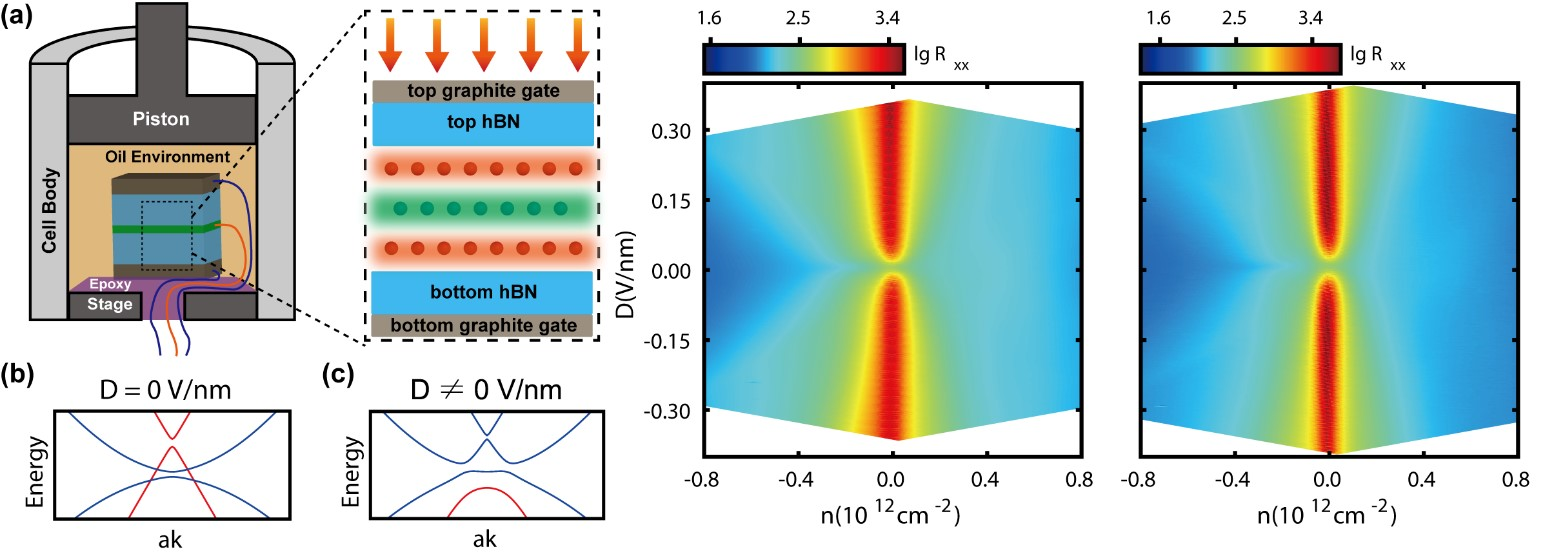
\includegraphics{figures/Figure_1.jpg}% Here is how to import EPS art
    \caption{\label{fig:1} Schematic of experimental setup and transport characterization.\\
    (a) Schematics of hydrostatic pressure setup. (b), (c) Schematics of How the displacement field influences the band structure of tri-layer ABA graphene.
    In the absence of displacement field D, the low energy bands include two monolayer-like bands with linear dispersion (red curve \& blue curve) 
    and two bilayer-like bands with parabolic dispersion (cyan curve \& green curve).
    When D is non-zero, these two bands hybridize, leading to a gap opening at the charge neutrality point, making the system insulate.
    (d), (e) device characterization before and after 1.0 GPa hydrostatic pressure by using the four-terminal longitudinal resistance $R_{xx}$ 
    as a function of carrier density $n(10^{12}cm^{-2})$ and displacement field D(V/nm). 
    Along the charge neutrality profile, the resistance increases dramatically as D increases, indicating a gap opening reflecting the device's good quality.
    }
\end{figure*}

\begin{figure*}
    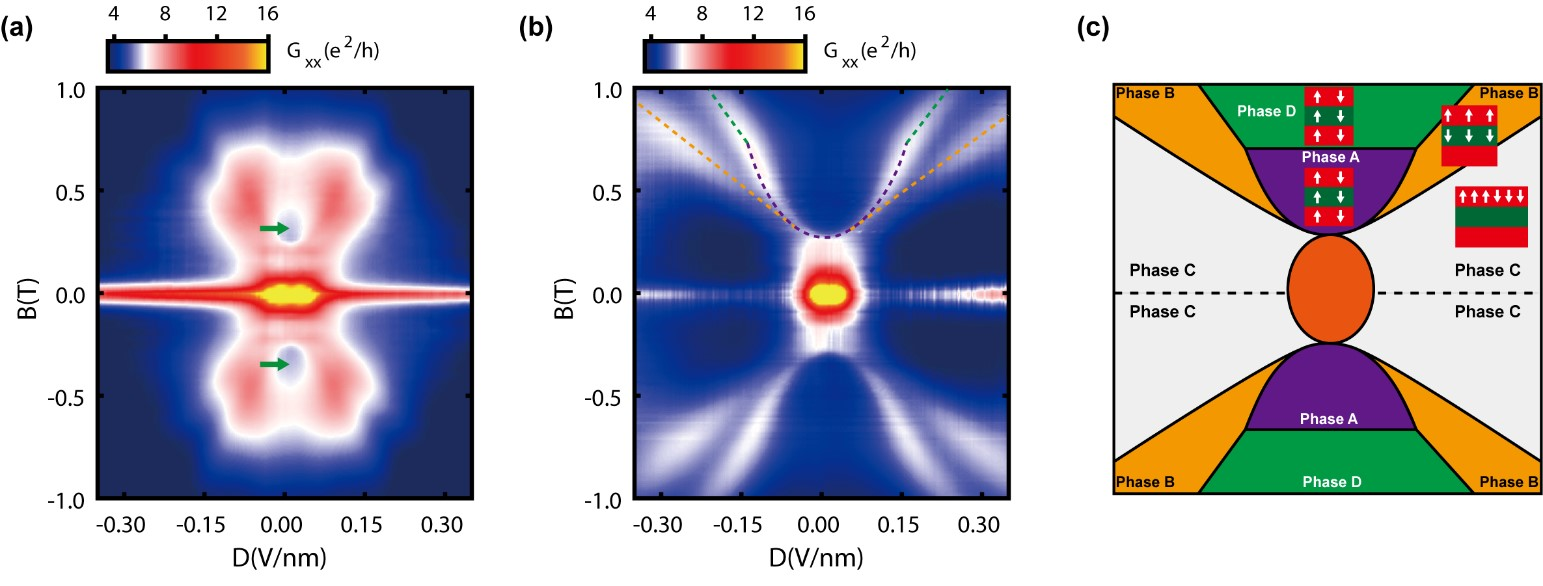
\includegraphics{figures/Figure_2.jpg}% Here is how to import EPS art
    \caption{\label{fig:2} Phase diagrams at the charge neutrality point before and after 1.0 GPa hydrostatic pressure.\\
    Here, Figures 2(a) and 2(b) show the phase diagrams of four-terminal longitudinal conductance $G_{xx}$ in unit of $\frac{e^2}{h}$ as a function of B(T) and D(V/nm), 
    with B ranges from -1.0 T to 1.0 T and D ranges from -0.30 V/nm to 0.30 V/nm, it is noted that the values larger than 16 has been rescaled to 16. 
    (a) shows the phase diagram at 0 GPa. A prominent feature emerges around D = 0 V/nm and B = 0.3T, indicated by the green arrow. 
    (b) the phase diagram at 1GPa shows visible traces of phase boundary (marked by dashed lines of different colours), 
    indicating first-order phase transitions between different ground states.
    This phase diagram is converted into a cartoon shown in (c). Different regions are filled with different colours, and specific phases are labelled with A, B, and C, 
    demonstrating the existence of different ground states.}
\end{figure*}

\begin{figure*}
    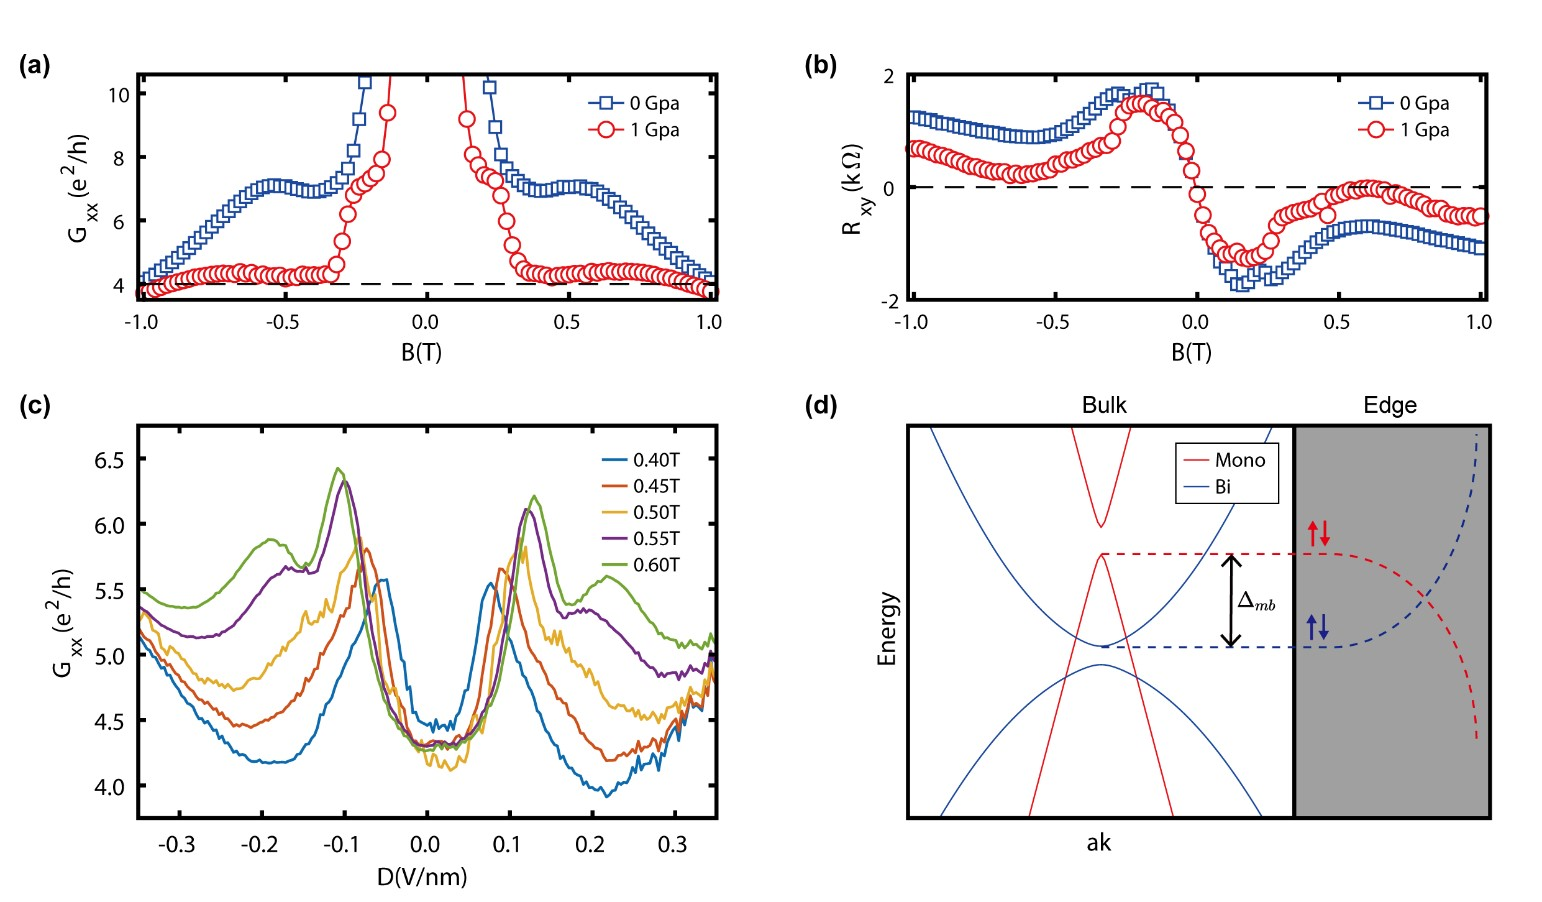
\includegraphics{figures/Figure_3.jpg}% Here is how to import EPS art
    \caption{\label{fig:3} Experimental signatures of Quantum Parity Hall effect and its schematics. \\
    (a) The longitudinal conductance $G_{xx}$ profiles of the D = 0 V/nm in both Figure~\ref{fig:2}(a) and ~\ref{fig:2}(b), blue squares mark the 0 GPa curve, 
    and red circles mark the 1 GPa curve. It can be seen that $G_{xx}$ becomes nearly quantized (about $4.1 \frac{e^2}{h}$) after pressure. 
    (b) The profiles of transverse resistance $R_{xx}$ at D = 0 V/nm, where the 1 GPa curve almost reaches zero around B = 0.6T, together with the nearly quantized signature in (a), 
    indicating the appearance of helical edge states in the system, which is the quantum parity hall state (QPHE). 
    (c) The profiles at B = 0.40 / 0.45 / 0.50 / 0.55 / 0.60 T are taken from Figure~\ref{fig:2}(b) as a function of displacement field D. The nearly quantized plateau disappears when D is large enough. 
    (d) The schematic of the mechanism of (QPHE) based on the band structure: the edge states from the monolayer valence band and that from the bilayer conduction band propagate along opposite directions 
    along the edge, and because of the spin degeneracy, there are four channels of edge states.
    }
\end{figure*}

% Table
\begin{table*}
\caption{\label{tab:table1}This is a table that records the fitting parameters at 0 Gpa and 1 Gpa based on the experimental results shown in figure.4(a)(b), \
the energy unit is set to $eV$. The intralayer hopping $\gamma_0$ is fixed as $3.100eV$.}
    \begin{ruledtabular}
        \begin{tabular}{ccccccccc}
            % &\multicolumn{2}{c}{$D_{4h}^1$}&\multicolumn{2}{c}{$D_{4h}^5$}\\
            Pressure & $\gamma_0$ & $\gamma_1$ & $\gamma_2$ & $\gamma_3$ & $\gamma_4$ & $\gamma_5$ & $\delta$ & $\Delta_2$ \\ \hline
            0 GPa & $3.100$ & $0.3845$ & $-0.0194$ & $0.3510$ & $0.0653$ & $0.0636$ & $0.0415$ & $0.0021$ \\
            1 GPa & $3.100$ & $0.3784$ & $-0.0234$ & $0.3665$ & $0.0612$ & $0.0833$ & $0.0534$ & $0.0031$ \\
        \end{tabular}
    \end{ruledtabular}
\end{table*}

\begin{figure*}
    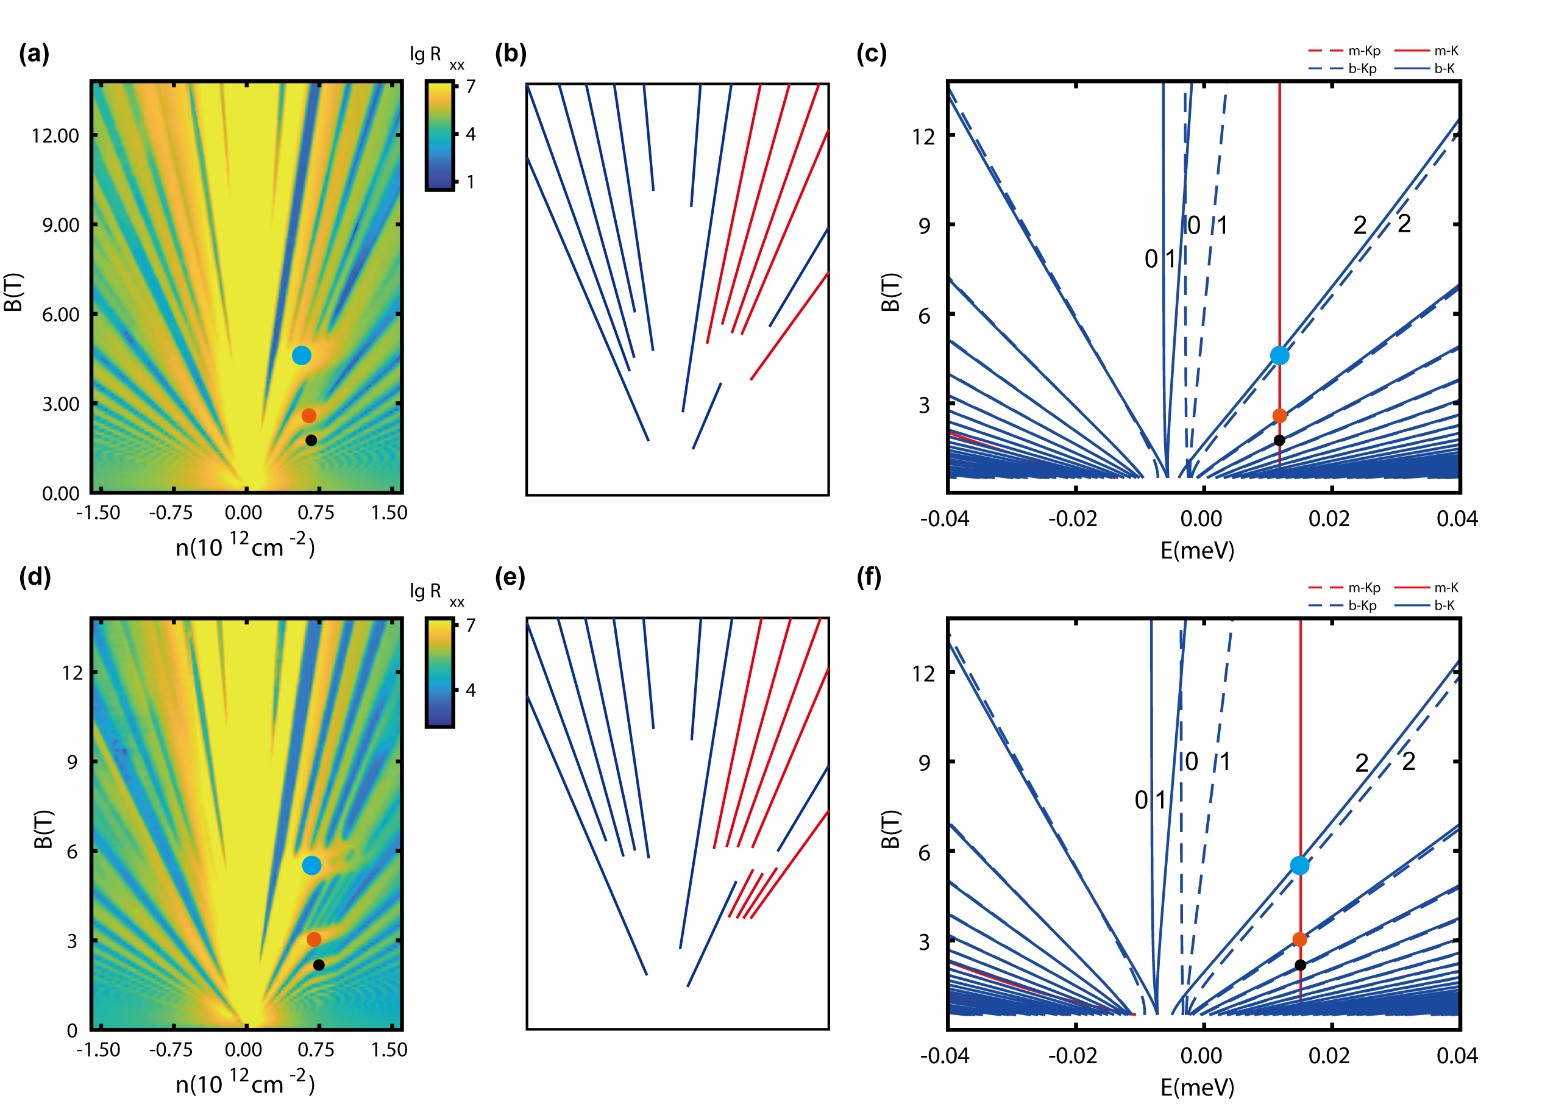
\includegraphics{figures/Figure_4.jpg}% Here is how to import EPS art
    \caption{\label{fig:4} Landau Fan diagrams at 0 GPa and 1 GPa, and the fitted simulation results.\\
    (a), (d) the Landau Fan diagrams at 0 GPa and 1 GPa, the crossing points between $(m, K/K^{\prime}, 0)$ and $(b, K^{\prime}, 2), (b, K^{\prime}, 3), 
    (b, K^{\prime}, 4)$ are marked by cyan, orange and black-coloured dots (P1, P2 and P3). It can be seen that the crossing points shift toward a large magnetic field 
    after pressure. In (b) (e), some minimum tracks at low integer fillings (from -6 to 10) are traced out, the blue colour indicates that the LLs are from a bilayer-like branch 
    while the red is from monolayer-like branch. (c), (f) the simulated Landau level structures fitted by the positions of crossing points from (a) and (b). 
    The corresponding points are also marked in the figures. The monolayer-like Landau levels are red-color, while the bilayer-like 
    Landau levels are blue-colour (dashed line for $K^{\prime}$ valley and solid line for $K$ valley). The numbers are the Landau level indexes in each branch. 
    The fitting parameters are listed in Table~\ref{tab:table1}.}
\end{figure*}

\end{document}
% Schematic of experimental setup and transport characterization.
% (a) Schematics of hydrostatic pressure setup. (b), (c) Schematics of How the displacement field influence the band structure of tri-layer ABA graphene. 
% When there is no displacement field D, the low energy bands include two monolayer-like bands with linear dispersion (red curve & blue curve), 
% and two bilayer-like bands with parabolic dispersion (cyan curve & green curve). 
% When D is non-zero, these two bands hybridize together, opening a gap at the charge neutrality point, making the system insulating. 
% (d), (e) device characterization before and after 1.0 GPa hydrostatic pressure by using the four-terminal longitudinal resistance $R_{xx}$ as a function of carrier density $n(10^{12}cm^{-2})$
% and displacement field D(V/nm).  
% These signatures demonstrate the good quality of our device.